\documentclass[ja=minimal]{bxjsarticle}
\usepackage{tikz}
\usepackage{luatexja}
\usepackage{luatexja-fontspec}


\usepackage{pgfplots}
\usepackage{amsmath}
\pgfplotsset{compat=1.18}
\usepackage{graphicx}
\usepackage{multicol}
\usetikzlibrary{intersections,calc,arrows.meta,angles,quotes,patterns}
\usepgfplotslibrary{fillbetween}

\begin{document}

\begin{center}
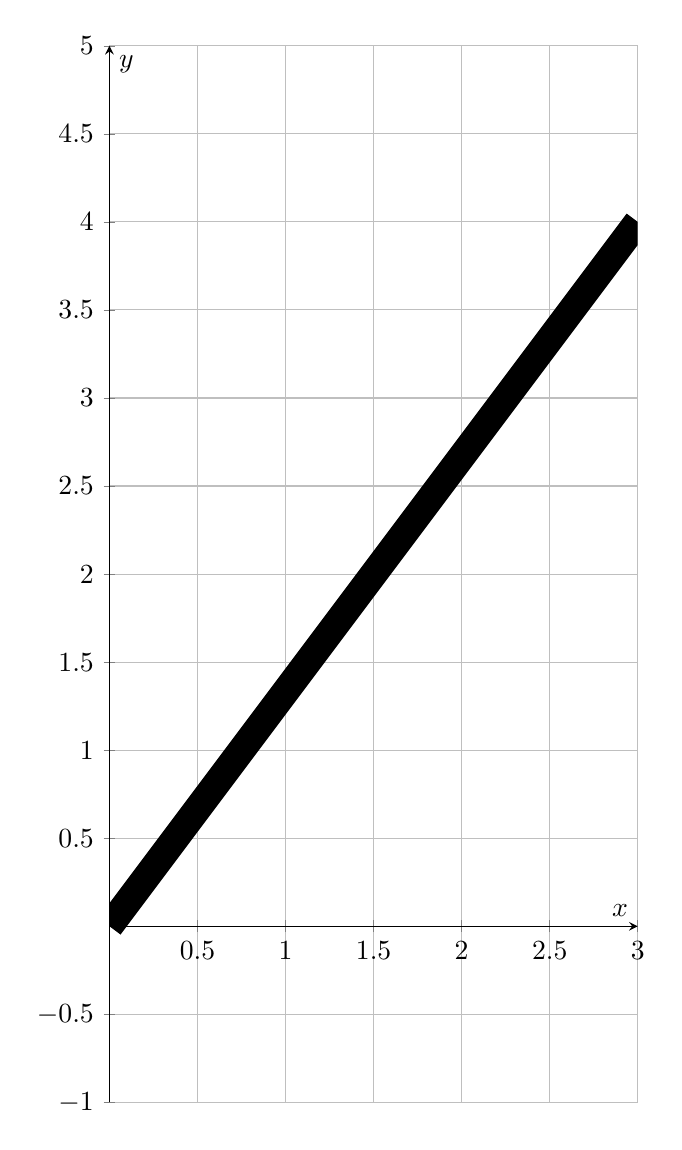
\begin{tikzpicture}

\begin{axis}[
            width=15cm,
            height=15cm,
            axis equal image,
            axis lines=middle,
            grid=major,
            enlargelimits=false,
            clip=true,
            xlabel=$x$,
            ylabel=$y$,
            domain=-1.0:5.0,
            ymin=-1.0,ymax=5.0,
            view={0}{90},
            samples=200
            ]
        
\addplot[line width=10pt, black] coordinates {({0.0},{0.0}) ({3.0},{4.0})};
\end{axis}
\end{tikzpicture}
\end{center}

\end{document}
